\documentclass{../lab}

\labacronym{CO$_2$}
\labtitle{CO$_2$ Laser}

%\newcommand{\ofOpticsTutorial}{http://experimentationlab.berkeley.edu/sites/default/files/QIE/fundamental-Optics.pdf}

\begin{document}

\maketitle

\tableofcontents

\section{CO\texorpdfstring{$_2$}{2} Laser Description (CO\texorpdfstring{$_2$}{2})}

\begin{enumerate}
    \item \textbf{Note that there is NO eating or drinking in the 111-Lab anywhere, except in rooms 282 \& 286 LeConte on the bench with the BLUE stripe around it.} Thank you -- the Staff.

\end{enumerate}

The carbon dioxide laser was the first high-powered infrared laser developed. The one in our laboratory is a new version that everything about it is something you can see, touch and adjust -- from filling the tube with gas, aligning the optical elements to measuring the output power and wavelengths. Its output can exceed 10 watts of monochromatic radiation, enough to burn you in a fraction of a second. So be careful with what you vary.

In this experiment, you will learn about molecular structure, light and optics, and gas discharges. You will develop skills in adjusting sensitive optical equipment. You will also learn how to work safely with electromagnetic radiation that you cannot see.

You MUST have a partner to do this experiment -- it takes two to align the laser cavity. You must schedule your time on successive days (no days off from the beginning to the end).

\begin{enumerate}
    \item Pre-requisites: Physics 137AB (137B may be taken concurrently)

    \item Days Allotted for the Experiment: 8

    \item Consecutive days: Yes

\end{enumerate}

\textbf{Warning From The Staff of the 111 Lab: DO NOT BURN any material like PAPER with the CO$_2$ Laser or put anything in the beam path that is not for this experiment.} We know you may want to do this but it is a safety hazard. You will receive a Grade of `F' for the experiment if you do so.

This lab will be graded 30\% on theory, 60\% on technique, and 10\% on analysis. For more information, see the \href{\AdvancedLabSyllabus}{\textbf{Advanced Lab Syllabus}}.

Comments: E-mail \href{\MailDonOrlando}{\textbf{Don Orlando}}

\section{The CO\texorpdfstring{$_2$}{2} Laser Experiment Photos}

\begin{figure}[!h]
\minipage{0.32\textwidth}
  \href{http://experimentationlab.berkeley.edu/sites/default/files/CO-2/CO2__4082B.jpg}{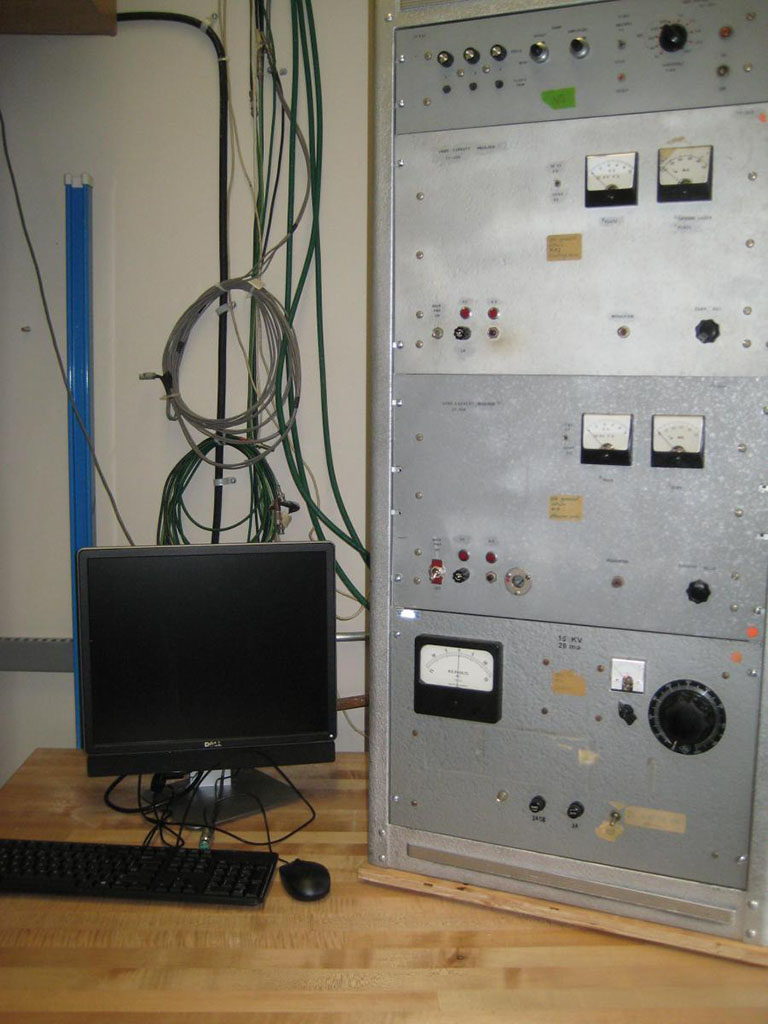
\includegraphics[width=\linewidth,keepaspectratio]{images/CO2__4082B.jpg}}
  \caption{High Voltage control board \\ \href{http://experimentationlab.berkeley.edu/sites/default/files/CO-2/CO2__4082B.jpg}{Click here to see larger picture}}
  \label{fig:HighVoltage}
\endminipage\hfill
\minipage{0.32\textwidth}
  \href{http://experimentationlab.berkeley.edu/sites/default/files/images/CO2_0687B.jpg}{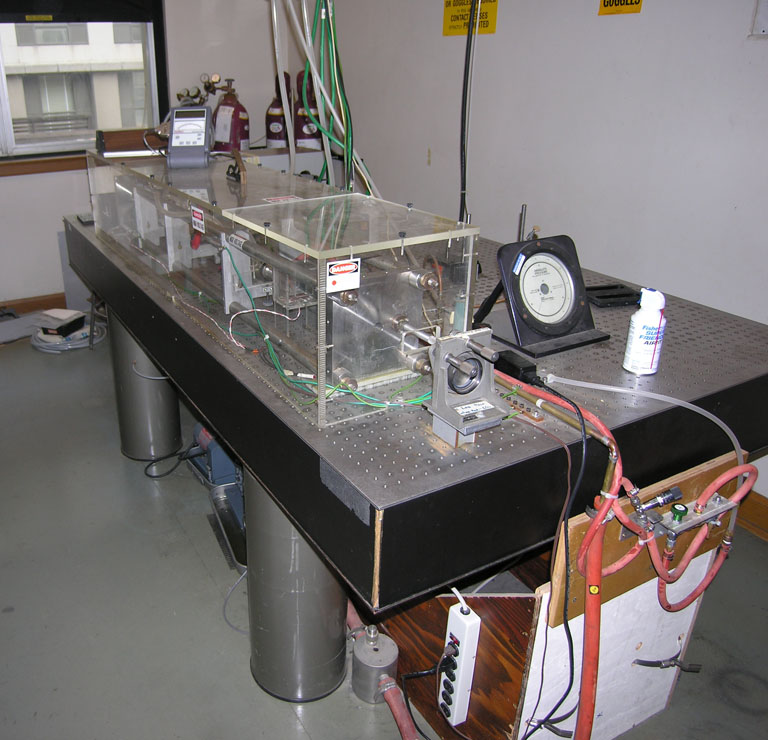
\includegraphics[width=\linewidth,keepaspectratio]{images/CO2_0687B.jpg}}
  \caption{CO$_2$ Laser Apparatus \\
  \href{http://experimentationlab.berkeley.edu/sites/default/files/images/CO2_0687B.jpg}{Click here to see larger picture}}
  \label{fig:LaserApparatus}
\endminipage\hfill
\minipage{0.32\textwidth}
  \href{http://experimentationlab.berkeley.edu/sites/default/files/CO-2/CO2_H2O_3529B.jpg}{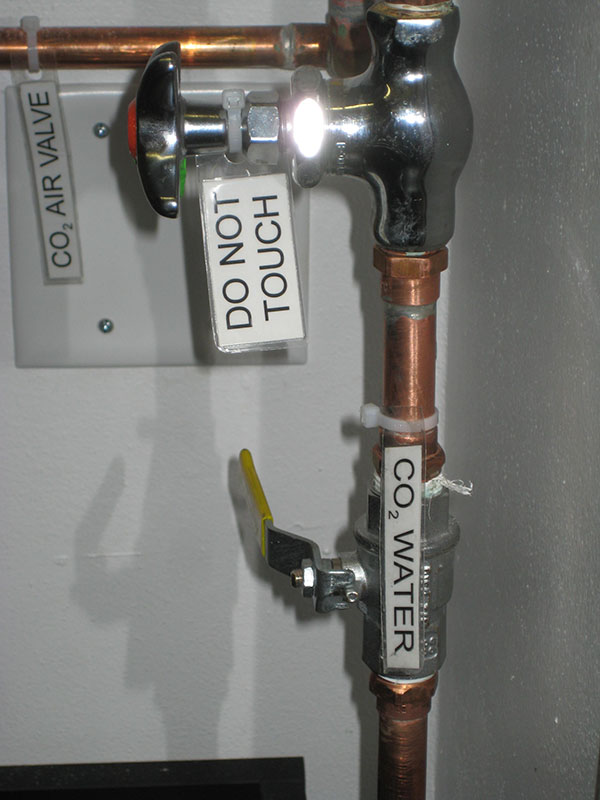
\includegraphics[width=\linewidth,keepaspectratio]{images/CO2_H2O_3529B.jpg}}
  \caption{Water valve \\ \href{http://experimentationlab.berkeley.edu/sites/default/files/CO-2/CO2_H2O_3529B.jpg}{Click here to see larger picture}}\label{fig:WaterValve}
\endminipage
\end{figure}

\begin{figure}[!h]
\minipage{0.32\textwidth}
  \href{http://experimentationlab.berkeley.edu/sites/default/files/images/CO2_Valves_3568.jpg}{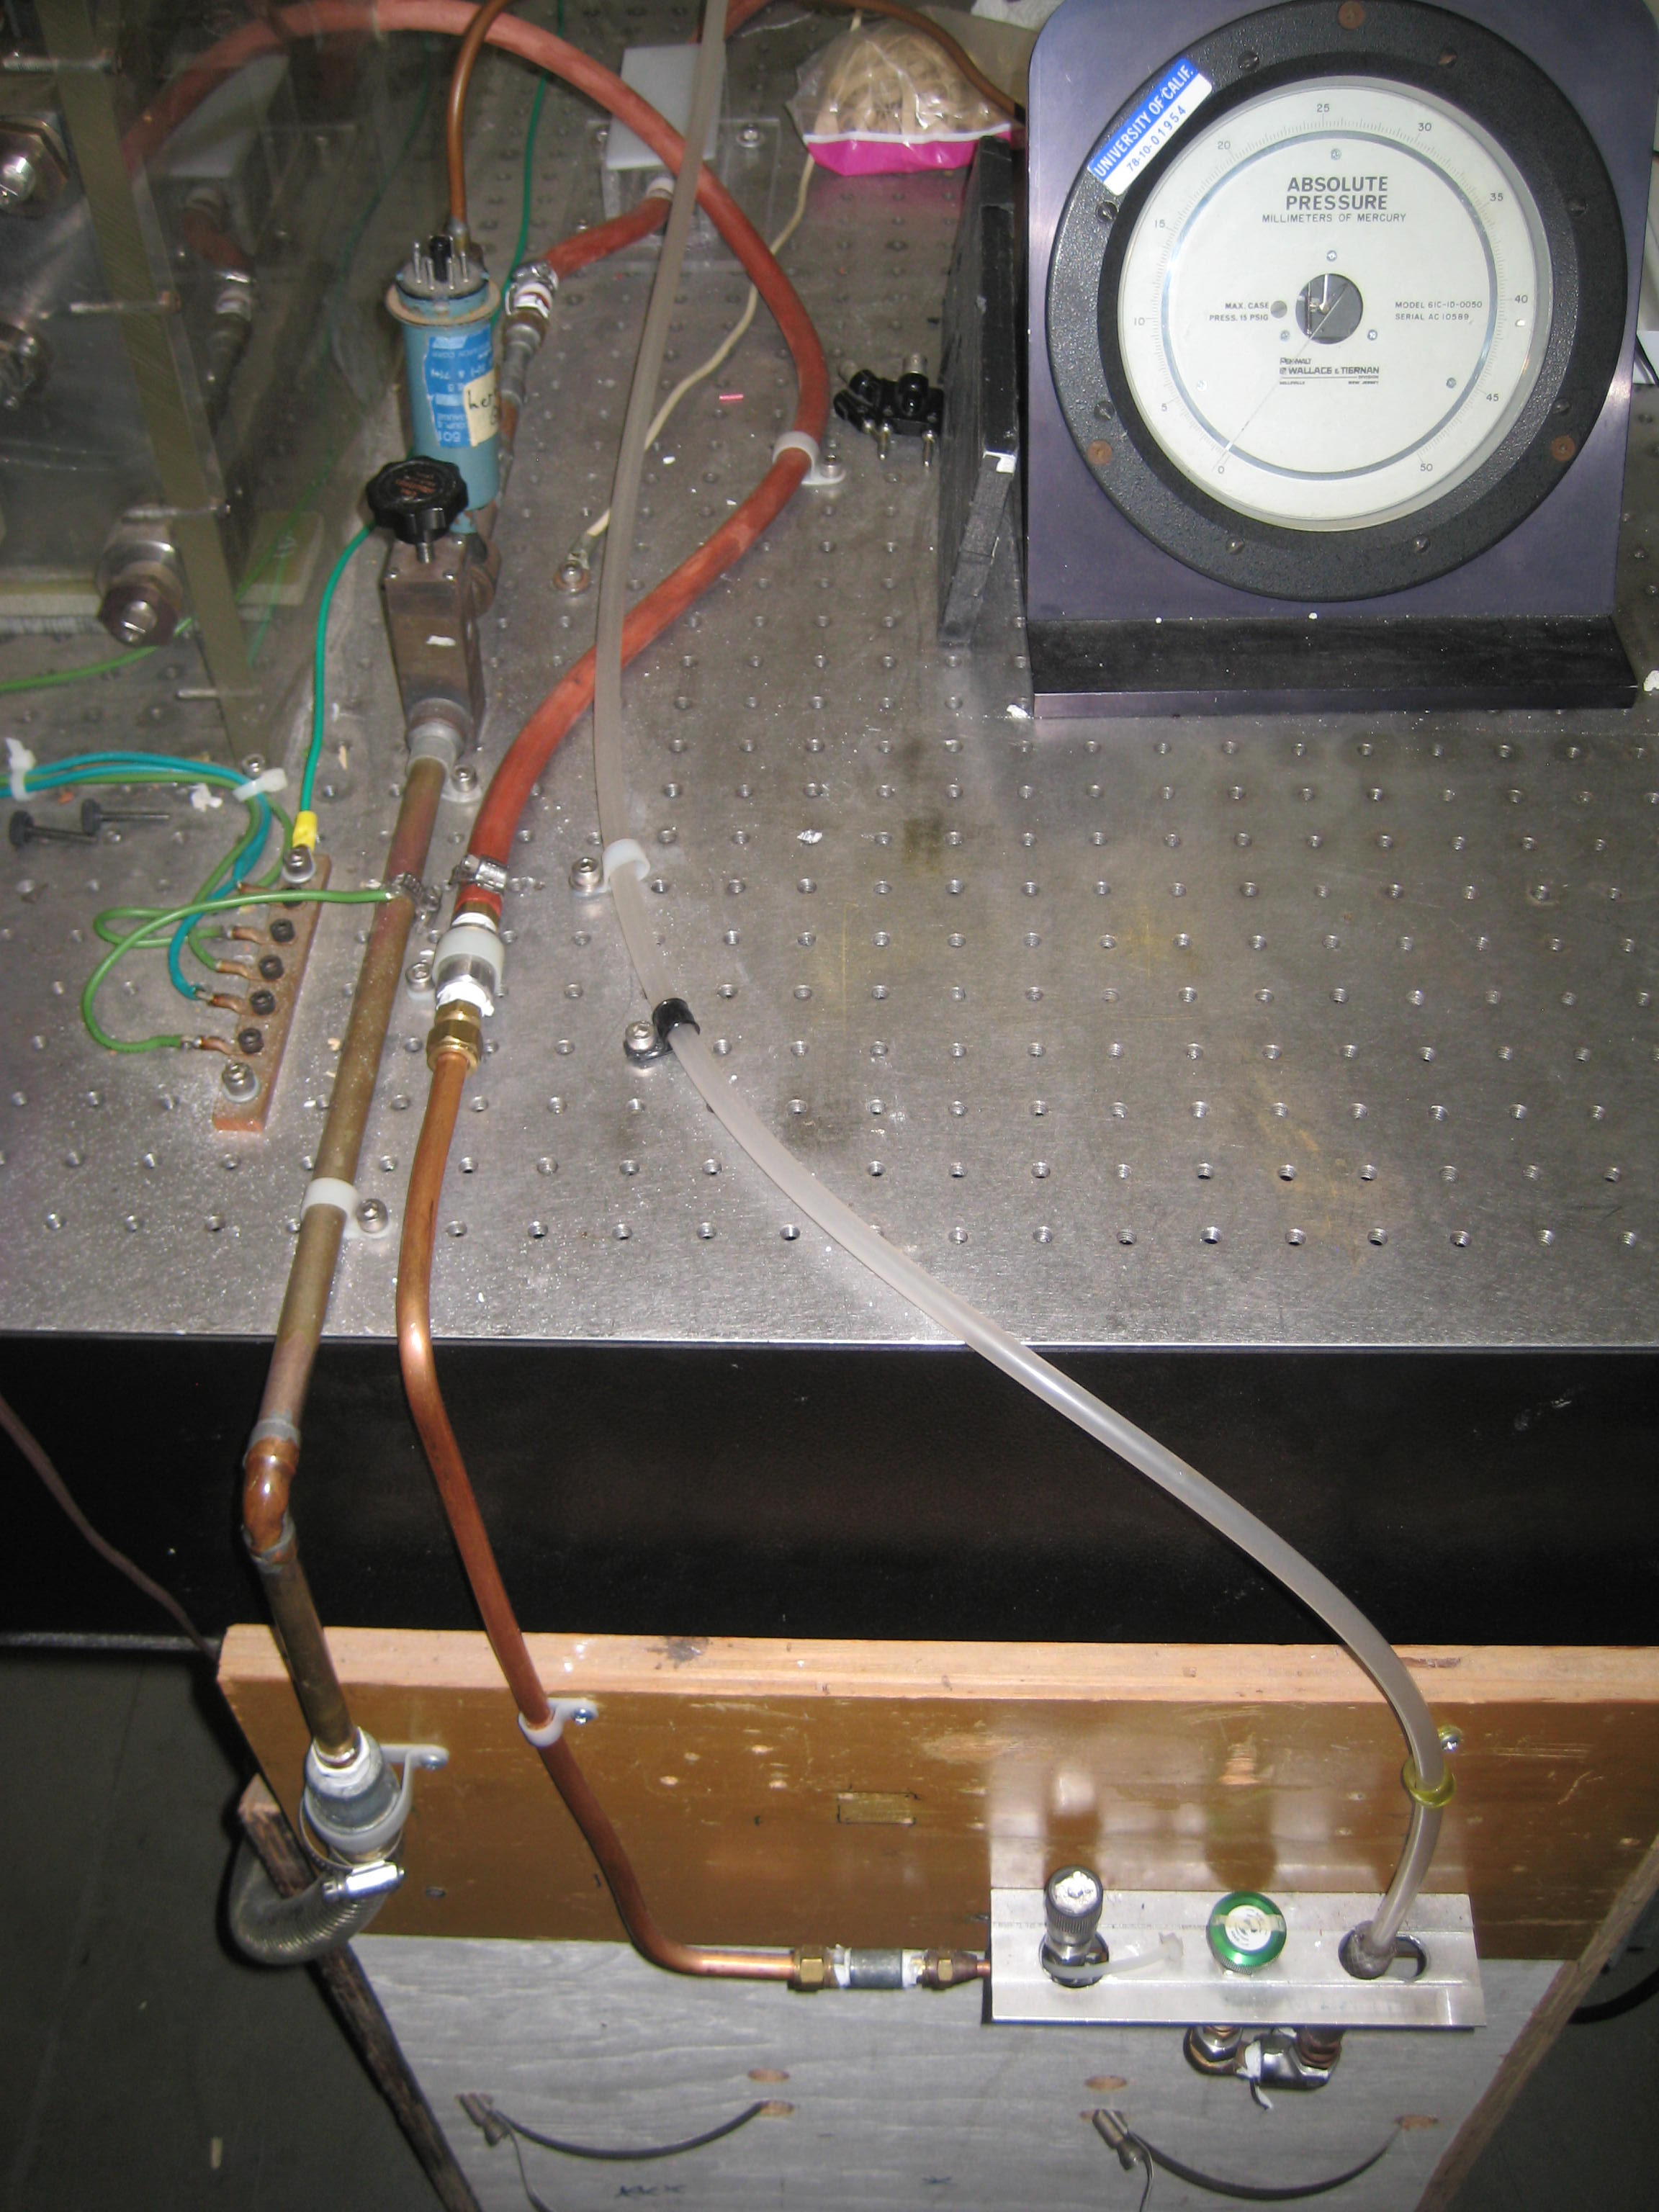
\includegraphics[width=\linewidth,keepaspectratio]{images/CO2_Valves_3568.jpg}}
  \caption{CO$_2$ valves\\ \href{http://experimentationlab.berkeley.edu/sites/default/files/images/CO2_Valves_3568.jpg}{Click here to see larger picture}}
  \label{fig:CO2Valves}
\endminipage\hfill
\minipage{0.32\textwidth}
  \href{http://experimentationlab.berkeley.edu/sites/default/files/images/Water_Drains_3531.jpg}{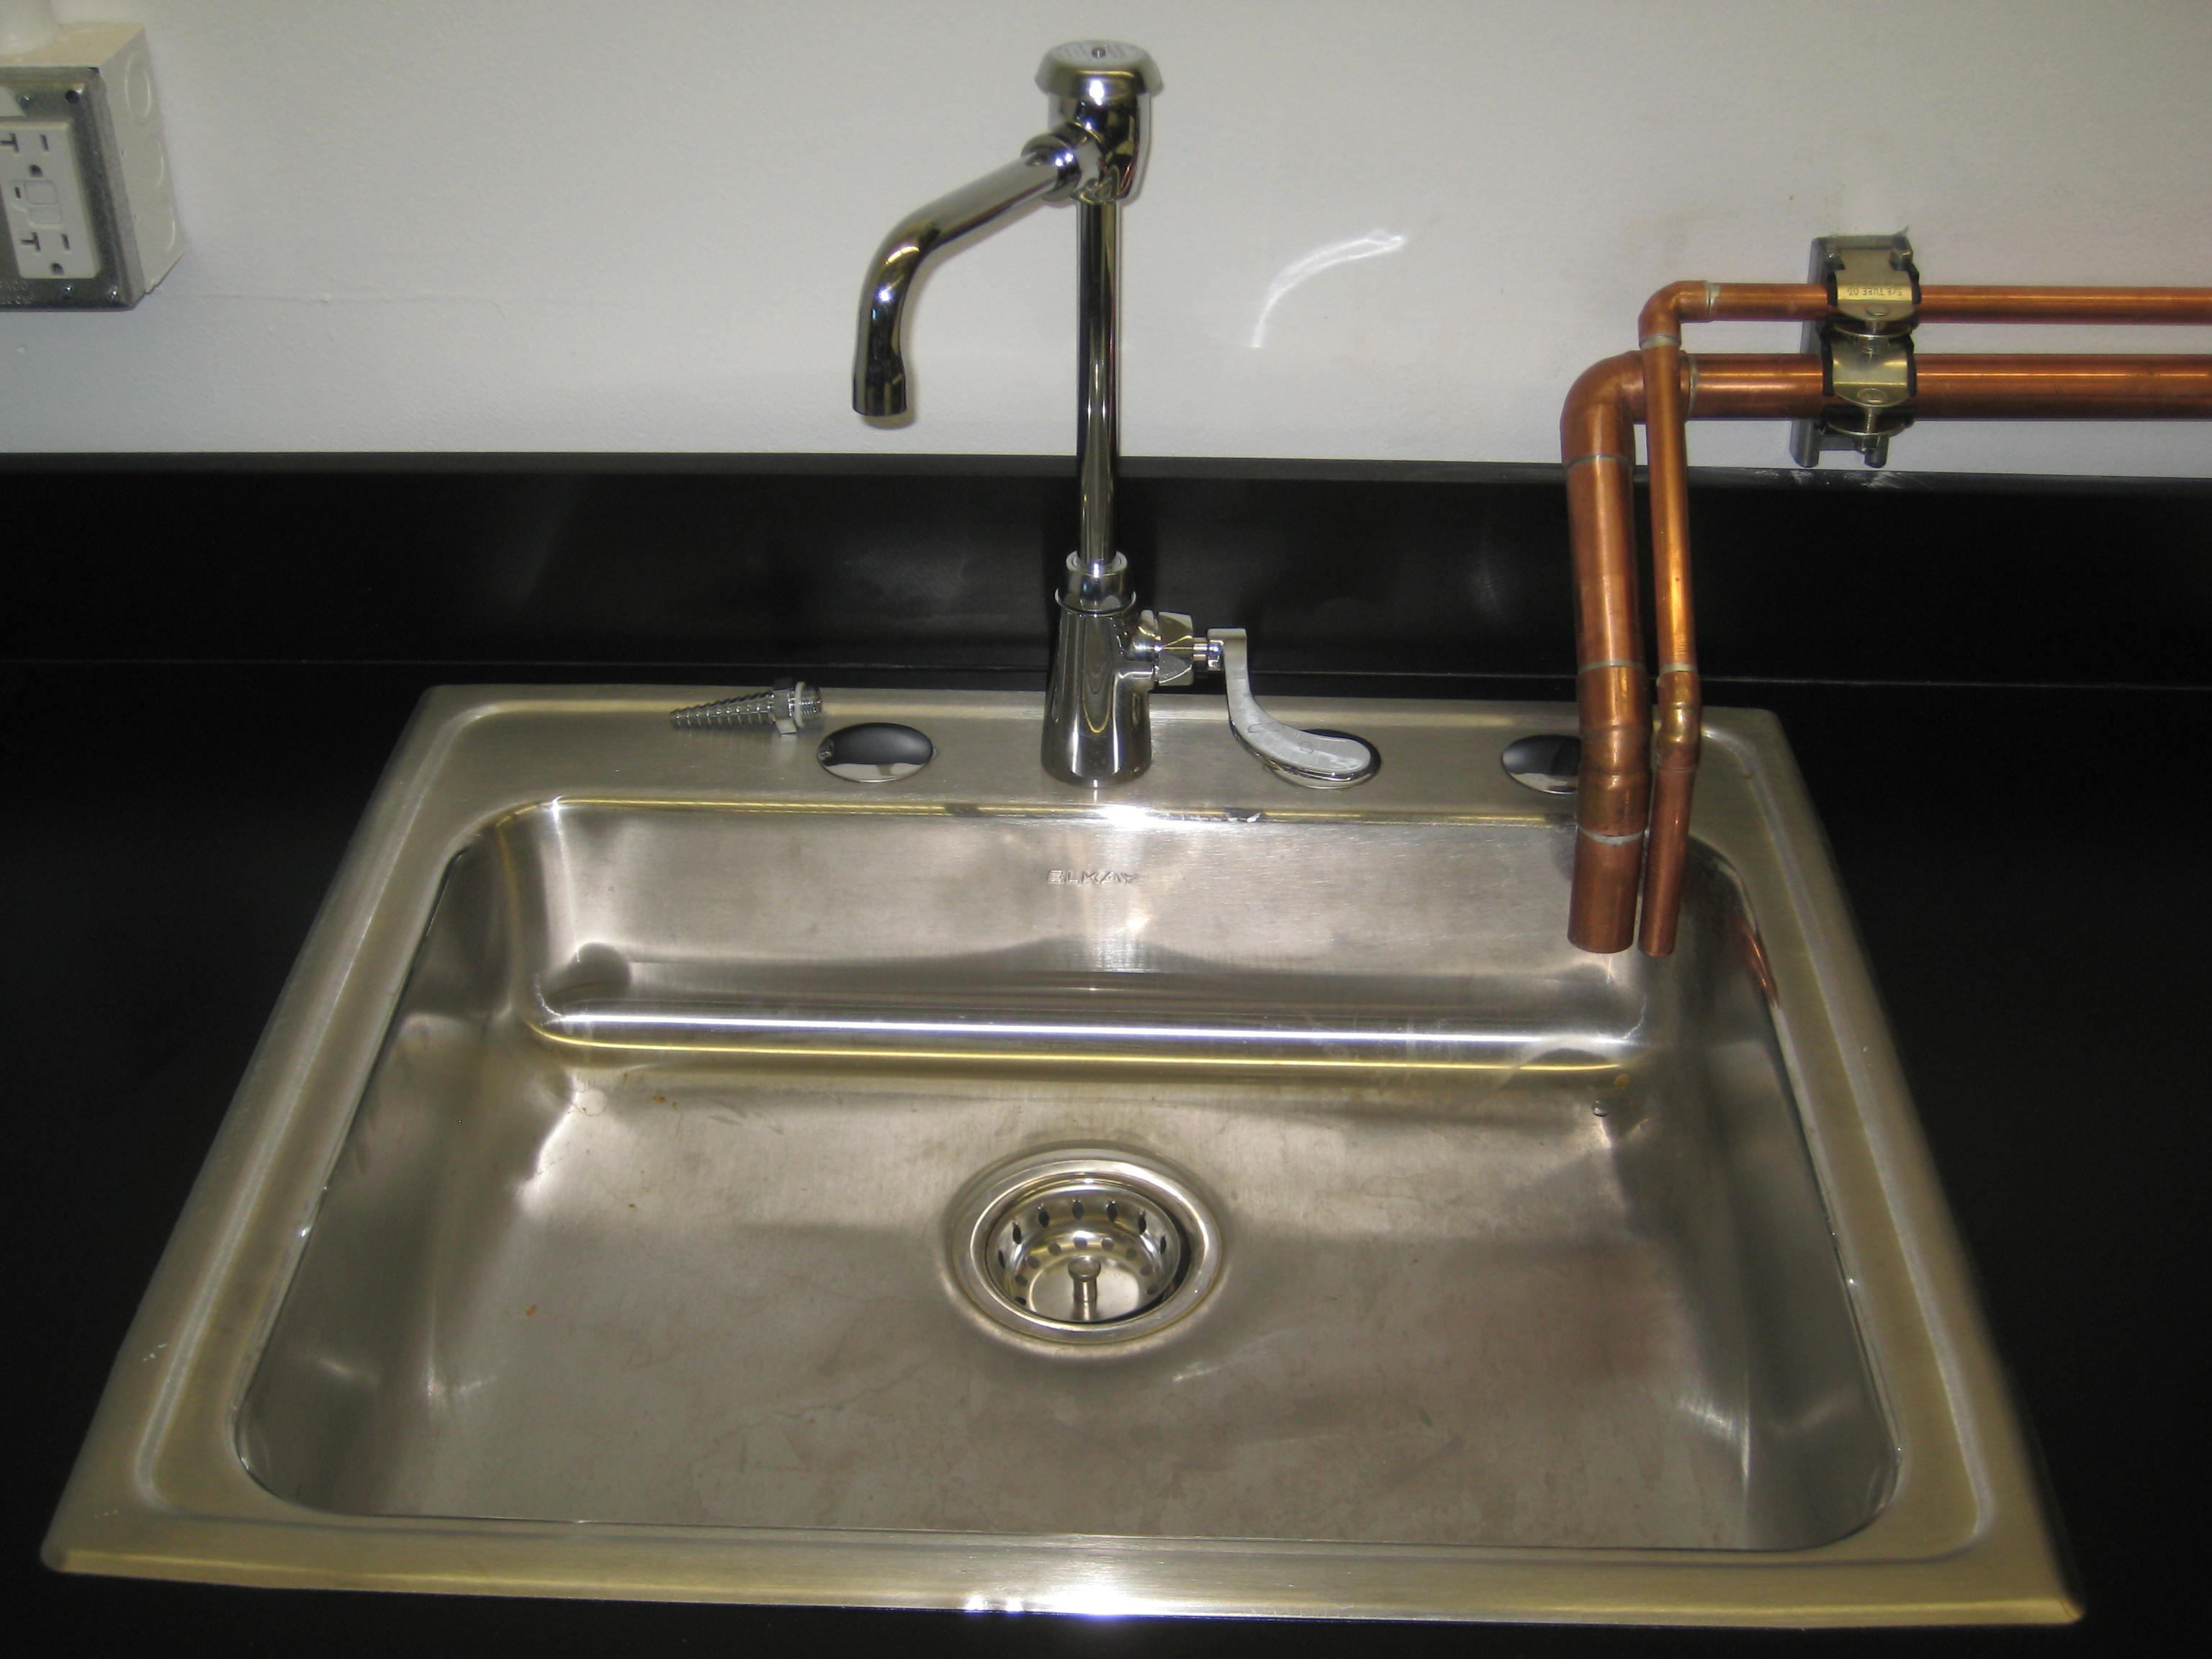
\includegraphics[width=\linewidth,keepaspectratio]{images/Water_Drains_3531.jpg}}
  \caption{Water drains \\
  \href{http://experimentationlab.berkeley.edu/sites/default/files/images/Water_Drains_3531.jpg}{Click here to see larger picture}}
  \label{fig:WaterDrains}
\endminipage\hfill
\minipage{0.32\textwidth}
  \href{http://experimentationlab.berkeley.edu/sites/default/files/images/HeNepower.jpg}{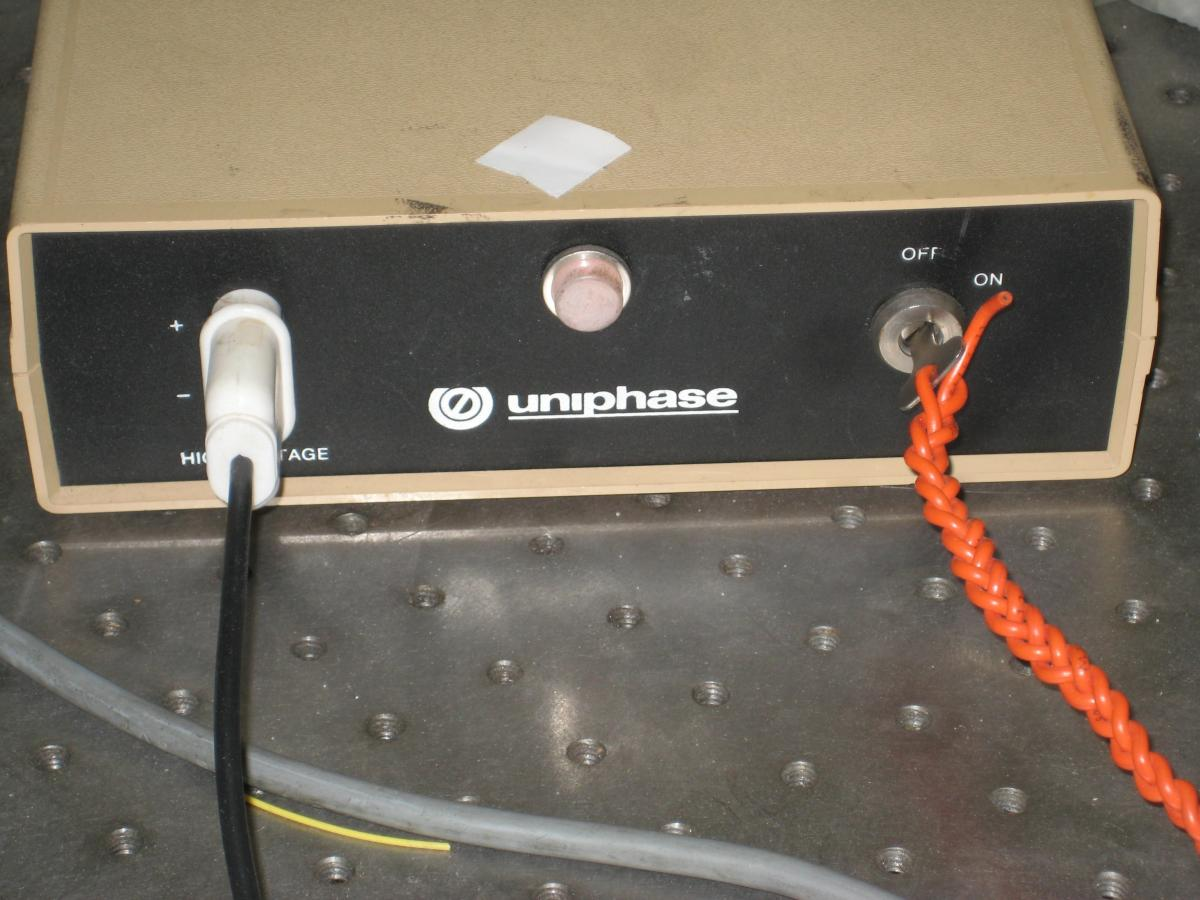
\includegraphics[width=\linewidth,keepaspectratio]{images/HeNepower.jpg}}
  \caption{Helium Neon laser power source \\ \href{http://experimentationlab.berkeley.edu/sites/default/files/images/HeNepower.jpg}{Click here to see larger picture}}\label{fig:HeNePower}
\endminipage
\end{figure}

\begin{figure}[!h]
\minipage{0.32\textwidth}
  \href{http://experimentationlab.berkeley.edu/sites/default/files/images/outputcoupler.jpg}{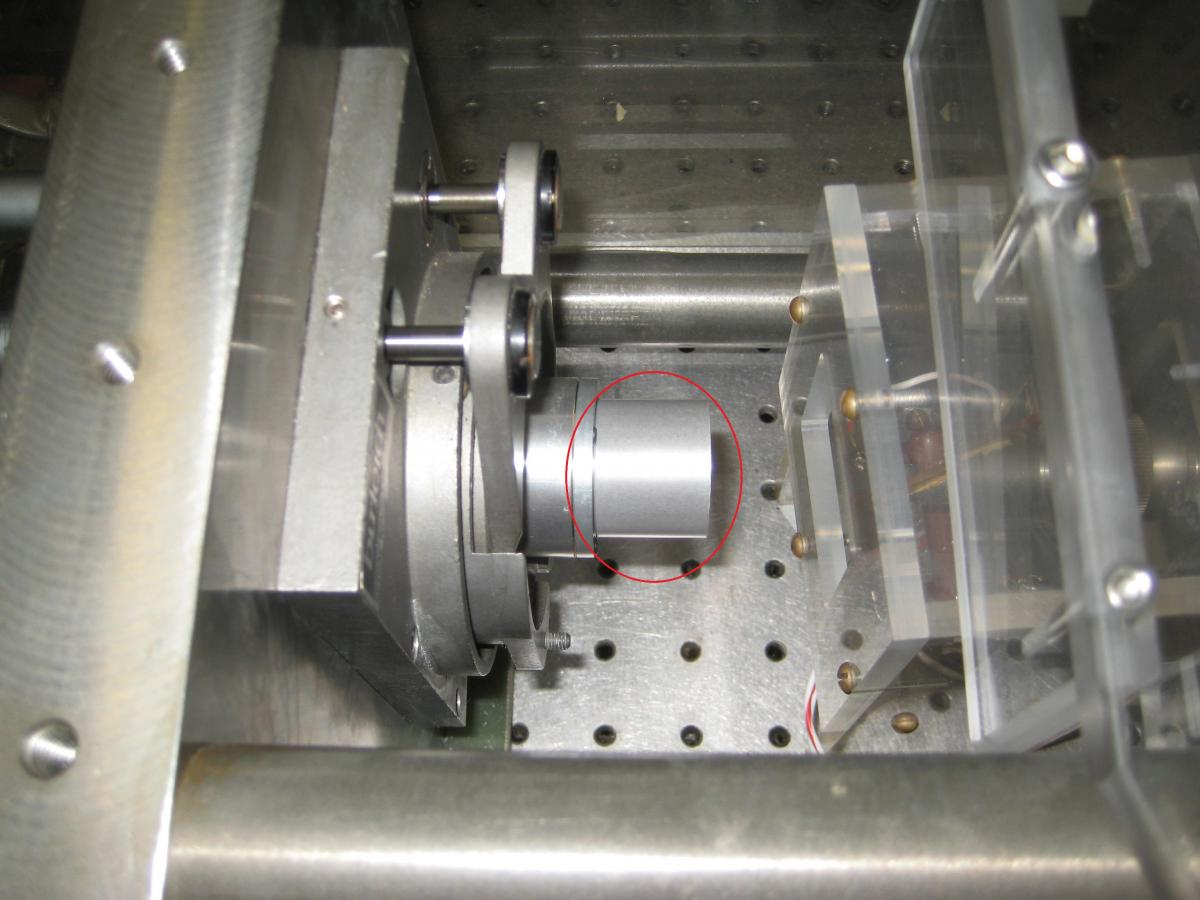
\includegraphics[width=\linewidth,keepaspectratio]{images/outputcoupler.jpg}}
  \caption{Output coupler\\ \href{http://experimentationlab.berkeley.edu/sites/default/files/images/outputcoupler.jpg}{Click here to see larger picture}}
  \label{fig:OutputCoupler}
\endminipage\hfill
\minipage{0.32\textwidth}
  \href{http://experimentationlab.berkeley.edu/sites/default/files/CO-2/CO2_Optics_3567_0.JPG}{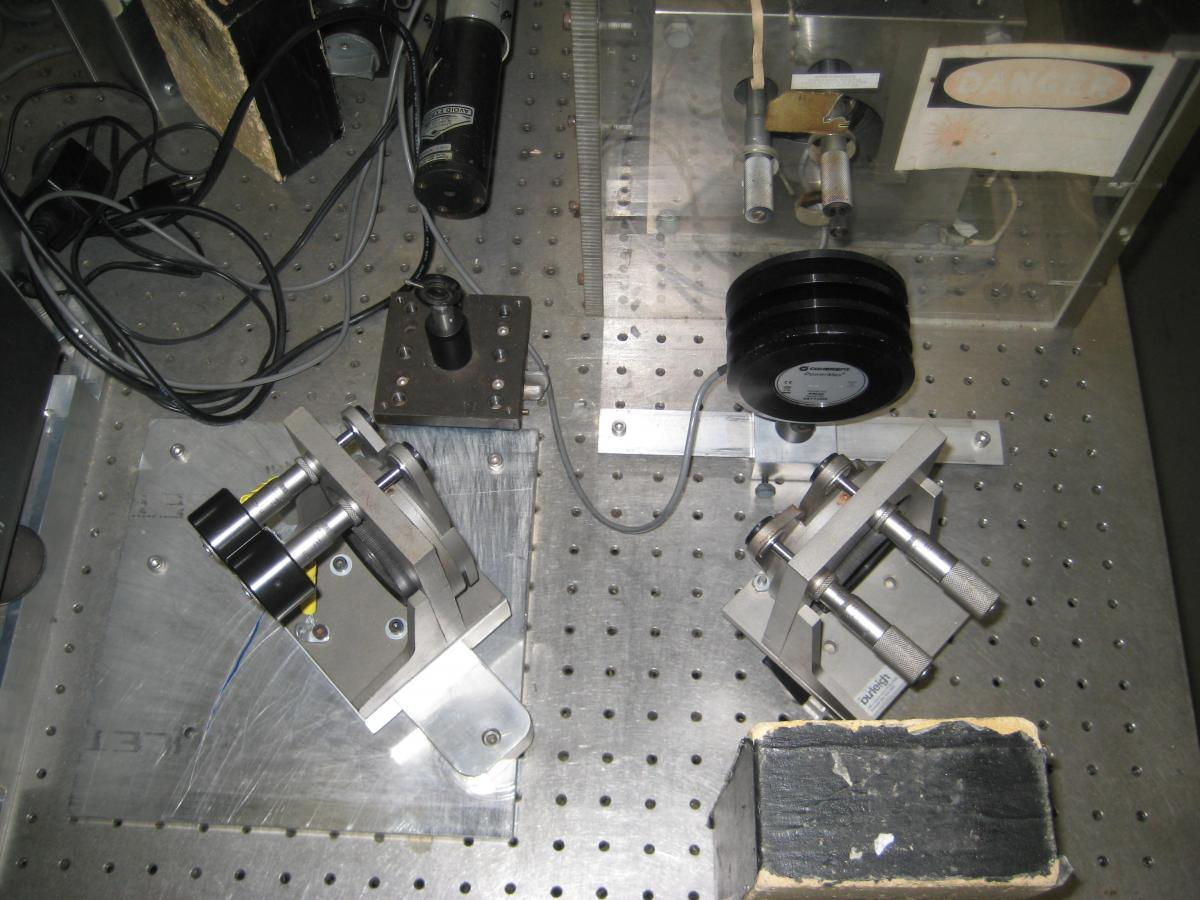
\includegraphics[width=\linewidth,keepaspectratio]{images/CO2_Optics_3567_0.JPG}}
  \caption{CO$_2$ optical alignment setup \\
  \href{http://experimentationlab.berkeley.edu/sites/default/files/CO-2/CO2_Optics_3567_0.JPG}{Click here to see larger picture}}
  \label{fig:OpticalAlignment}
\endminipage\hfill
\minipage{0.32\textwidth}
  \href{http://experimentationlab.berkeley.edu/sites/default/files/CO-2/Co-2-Grating_3641_0.JPG}{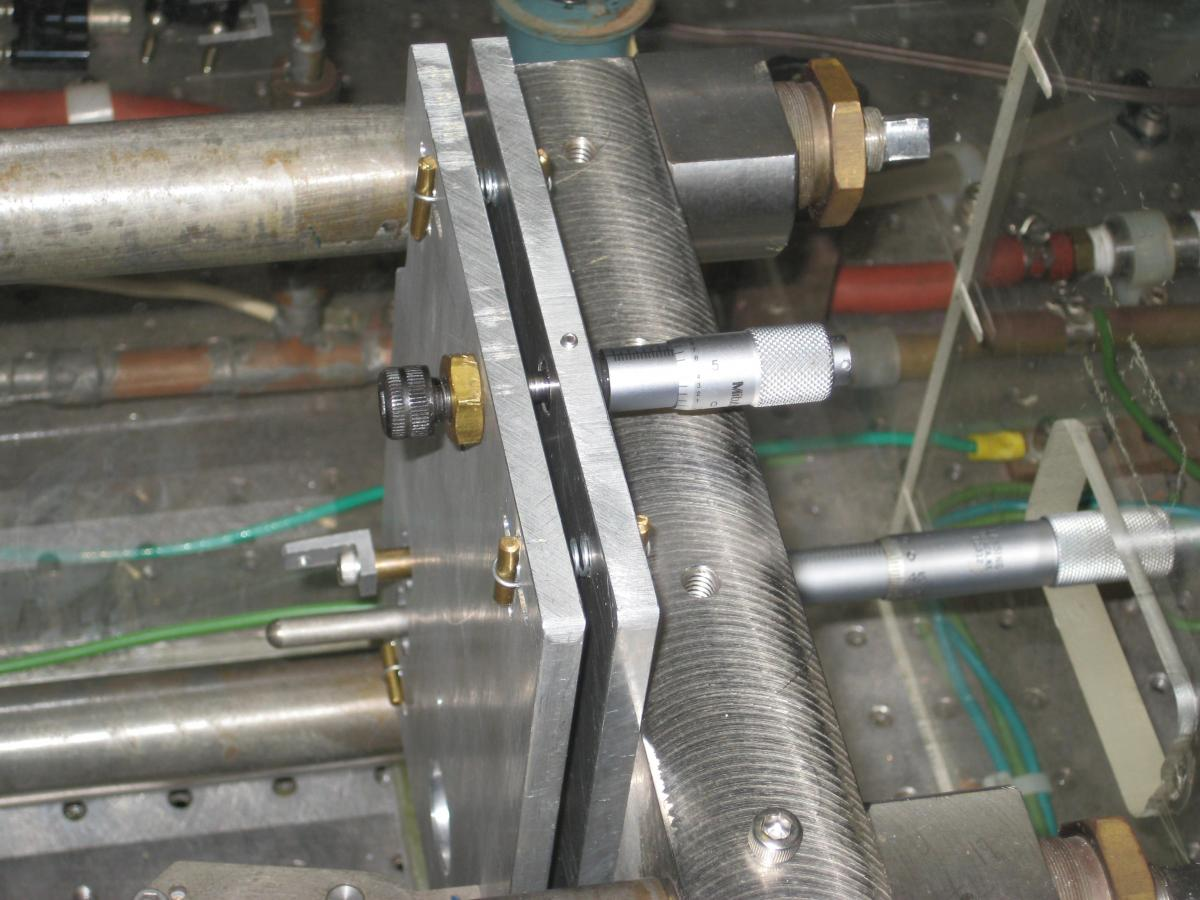
\includegraphics[width=\linewidth,keepaspectratio]{images/Co-2-Grating_3641_0.JPG}}
  \caption{CO$_2$ grating \\ \href{http://experimentationlab.berkeley.edu/sites/default/files/CO-2/Co-2-Grating_3641_0.JPG}{Click here to see larger picture}}\label{fig:Grating}
\endminipage
\end{figure}

\pagebreak

\section{Before the 1st Day of Lab}

\textbf{Complete the following before your experiment's scheduled start date:}

\begin{enumerate}
    \item \emph{\textbf{Note: In order to view the private Youtube videos hosted by the university, you must be signed into your berkeley.edu Google account.}} \\
    View the \href{http://youtu.be/-cLSnuXGC\_U}{\textbf{CO$_2$ Laser Video}}.

    \item Checkpoints are examination points where you must STOP and get a GSI or professor to verify your understanding and/or verify proper experimental setup. You cannot skip the checkpoints, as there is a \href{http://experimentationlab.berkeley.edu/node/137}{\textbf{sign off sheet}} that must be scanned in with your lab report. Print out the checkpoints page now and look it over.

    \item Before using the apparatus in this experiment, you must complete training in the safe use of lasers detailed on the \href{http://experimentationlab.berkeley.edu/lasersafety}{\textbf{\textbf{Laser Safety Training page}}}. This includes readings, watching a video, taking a quiz, and filling out a form.

    \item Complete the \href{http://experimentationlab.berkeley.edu/CO2prelab}{\textbf{\textbf{CO$_2$ Pre Lab and Evaluation}}} sheets. Print,  fill out with the answers and turn it in with your report. The Pre-Lab must be printed separately. Discuss the experiment and pre-lab questions with any faculty member or GSI and get it signed off by that faculty member or GSI. Turn in the signed pre-lab sheet with your lab report.

    \item Review the principles of optics, view the \href{http://experimentationlab.berkeley.edu/sites/default/files/QIE/fundamental-Optics.pdf}{\textbf{Fundamentals of Optics Tutorial}}, the \href{http://youtu.be/zUGBt5vc5FA}{\textbf{Optical Instruments Video}}, \href{http://youtu.be/wyBOVjU5bBQ}{\textbf{Energy Levels (part 1) Video}}, \href{http://youtu.be/Eypw0DmVBxk}{\textbf{Energy Levels (part 2) Video}}, and \href{http://youtu.be/xOMgdVP3AfE}{\textbf{Transitions video}}.

    \item Last day of the experiment please fill out the \href{\ExperimentEvaluation}{\textbf{Experiment Evaluation}}

\end{enumerate}

\noindent\textbf{Suggested Reading:}

\begin{enumerate}
    \item C. Patel, \emph{``}\href{http://physics111.lib.berkeley.edu/Physics111/Reprints/CO2/01-High\_Power\_Carbon\_Dioxide\_Lasers.pdf}{\textbf{High Power Carbon Dioxide Lasers}}\emph{''}, \emph{Scientific American}, August. 1968: an excellent introduction to the CO$_2$. laser.

    \item A. Bloom, ``\href{http://physics111.lib.berkeley.edu/Physics111/Reprints/CO2/CO2\_ch1\_A\_Bloom\_Basic\%20Principles.pdf}{\textbf{Ch.1: Basic Principles}}'' \emph{Gas Lasers}. Pp 1-42. John Wiley \& Sons Inc. New York. 1968; a good, readable book, especially on resonators.

    \item C. Garrett, \emph{\href{http://physics111.lib.berkeley.edu/Physics111/Reprints/CO2/CO2\%20OCR\%20Gas\%20Lasers\%20Garrett\%20pg.\%2011-82.pdf}{\textbf{Gas Lasers}}}, Pp: 11-82. McGraw Hill. San Francisco. 1967: a basic treatment of cavities, excitation mechanisms, and other topics.

    \item B. Lengyel, \emph{\href{http://physics111.lib.berkeley.edu/Physics111/Reprints/CO2/02-Gas\_Lasers.pdf}{\textbf{Lasers}}}, 2nd ed., 1971: a very good introduction to lasers in general, with a good section on CO$_2$ lasers.

    \item D. Sinclair and W. Earl Bell. ``\href{http://physics111.lib.berkeley.edu/Physics111/Reprints/CO2/CO2\%20\%20OCR\%20ch1\%20and\%202\_Sinclair\_Bell.pdf}{\textbf{Ch. 1: Introduction and Ch. 2: Interaction of Radiation and Matter}}.'' \emph{Gas Laser Technology}. Pp: 1-35. Holt, Rinehart, and Winston Inc. San Francisco. 1969: gives a readable theoretical treatment of laser physics.

    \item Cheo, P.K. ``\href{http://physics111.lib.berkeley.edu/Physics111/Reprints/CO2/03-CO2\_Lasers.pdf}{\textbf{Chapter 2: CO$_2$ Lasers.}}'' \emph{Lasers} edited by: A. Levine and A. DeMaria. Vol. 3, 1971: contains a comprehensive and detailed review article and lists many references.

    \item A. Levine, ``\href{http://physics111.lib.berkeley.edu/Physics111/Reprints/Lasers\%20Vol\%202\%20Levine/Chapter\%201\%20Gas\%20lasers\%20CKN\%20Patel.pdf}{\textbf{Chapter 1: Gas Lasers}}.'' \emph{Lasers}, vol. 2: contains a review article by Patel.

    \item A. Yariv. ``Chapters 7, 8, 9, 10.'' \href{http://physics111.lib.berkeley.edu/Physics111/Reprints/CO2/Quantum\_Electronics2ed\_A-Yariv/CO2\_Quantum\%20Electronics\_index.html}{\textbf{Quantum Electronics}}, 2nd ed., 1975: practical laser physics in more mathematical detail; the place to look when you need a formula, for example, to describe resonator properties.

    \item R.J. Pressley, \emph{\href{http://physics111.lib.berkeley.edu/Physics111/Reprints/CO2/PRESSLEY\_Lasers/CO2\_Pressley\%20Lasers\_index.html}{\textbf{CRC Handbook of Lasers}}}, 1971. Has a very brief description of CO$_2$ laser spectroscopy and lists wavelength data and references.

    \item G. Herzberg, \emph{\href{http://physics111.lib.berkeley.edu/Physics111/Reprints/ATM/02-2ndEd-Atomic\_Spectra\_and\_Atomic\_Structure.pdf}{\textbf{Introduction to Atomic Spectra}}}, vol. 2, 1945. The classic work on spectroscopy. Lists wavelength data and references.

    \item \href{http://experimentationlab.berkeley.edu/sites/default/files/pdfs/CO\_2\%20Energy\%20Levels.pdf}{\textbf{CO-2 Energy Levels}}

\end{enumerate}

More \hyperref[sec:References]{References}

[\href{\LabReprints}{\textbf{Physics 111 Library Site}}]

You should keep a laboratory notebook. The notebook should contain a detailed record of everything that was done and how/why it was done, as well as all of the data and analysis, also with plenty of how/why entries. This will aid you when you write your report.

\section{Objectives}

\begin{itemize}
    \item Learn what real experimental physics is about

    \item Learn the synergy between experimental and theoretical work

    \item Learn to use pieces of equipment that are commonly used in research

    \item Learn how measurements are performed, analyzed, and interpreted.

    \item Learn how to present your work and results

    \item Learn problem solving strategies

    \item Learn how to manage and organize your time

\end{itemize}

\section{Introduction}

The central piece of the equipment and object of study in this experiment is a continuous-wave (CW) carbon dioxide laser. It is of relatively low power as CO$_2$ lasers go, but is still capable of generating 10 W CW output, or roughly 1000 times the power of a small He-Ne laser. It operates in the infrared at a wavelength near $10^{-6}$ m and so is outside the human visual range. High power + invisible radiation + the presence of high voltage make it potentially very hazardous. SAFETY MUST BE YOUR MAJOR CONCERN AT ALL TIMES. Safety measures are detailed in the next section. If you ever have any doubt about some procedure, consult a professor, GSI, or Don Orlando.

\subsection{Safety Measures}

\begin{enumerate}
    \item Never operate anything, especially alone, unless you know exactly what you are doing. Anytime you don't understand something, ask for assistance. Protective eye goggles are available for UV and IR.

    \item The high voltage should never be turned on unless
    \begin{enumerate}
        \item all connections are secure;

        \item the water is flowing.

        \item \emph{\textbf{The gas is flowing through the laser!}}

    \end{enumerate}

    \item The laser beam must never be uncontrolled. This means:
    \begin{enumerate}
        \item when powering up the laser, the output should be blocked with the power detector and a firebrick; always include the firebrick.

        \item beam finders, optical pieces, and anything else must be inserted in the beam with great care, and in such a way that there can be no damage to the object or the person, and that the beam is not reflected or scattered in an unintended direction;

        \item place firebricks behind mirrors and detectors as backup protection.

        \item never let the beam probes set in the laser beam for more than 5 seconds; keep them moving in and out of the beam.

    \end{enumerate}

    \item NO UNAUTHORIZED PERSONS ARE ALLOWED AROUND THE APPARATUS. No casual visitors nor anyone not enrolled in the 111 Lab is allowed in the room. Step outside when you talk to them.

    \item In the event of an accident, the first thing to do is to shut off the high voltage at the current regulator and the high-voltage power supply. Then shut off BOTH WATER VALVES. (BLUE AND RED handles on the wall by the door. BLUE first; RED second.) Then call the 111-lab personnel for help.

\end{enumerate}

\section{Equipment}

The table on which the CO$_2$ laser sits is an optical table resting on four air-filled legs to isolate the laser from room and building vibrations. The table is always filled with 50 pounds of regulated air pressure. If an air line breaks please quickly call for help. The main shut-off valve labeled `CO$_2$ Air' is on the wall behind the Atomic Physics experiment in room 286.

\begin{figure}[h]
    \centering
    \href{http://experimentationlab.berkeley.edu/sites/default/files/images/CO23.gif}{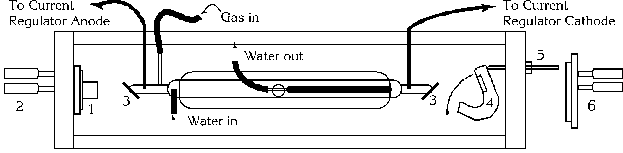
\includegraphics[width=0.7\linewidth]{images/CO23.png}}
    \caption{The Laser (top view)}
    \label{fig:TheLaserTopView}
\end{figure}

\begin{enumerate}
    \item Output-Mirror assembly: Mirror is ZnSe, 91\% reflectivity, 10 m radius of curvature.

    \item Horizontal and Vertical output mirror adjustments
    
    \item NaCl Brewster-angle windows
    
    \item 75 grooves/mm grating on a swivel mount
    
    \item Grating adjustment
    
    \item Totally reflecting back mirror with Horizontal and Vertical adjustments
\end{enumerate}

\section{Standard Operation Procedure (SOP) for the CO\texorpdfstring{$_2$}{2} Laser}

Before you start, familiarize yourself with the various pieces of apparatus. Look at the power meter to see how it operates and \textbf{turn it off when not in use}. Identify the HeNe or Diode laser used for alignment, firebrick, spectrum analyzer for the CO$_2$ spectrum, gas filling system with tank, regulators, valves, pressure gauges, high-voltage power supply and current regulator. When you work, keep the working surface neat and free of unused apparatus; this is good laboratory practice and an important safety measure.

\begin{enumerate}
    \item \textbf{Now put on a pair of the safety goggles}. Then turn on the HeNe laser and look for stray beams emanating off of any surfaces or optics. The CO$_2$ laser will be reflecting in the same places and in the same way only you cannot see the beam. Align the mirrors on the CO$_2$ Laser. Then when you turn on the CO$_2$ Laser perform a survey of the laser beam paths to check if there are any stray beams (diffuse or specular) with the beam probes. (Note that the higher the number on the beam probe the more sensitive the beam probe, check the references). Document your survey in the log book that is located in the wall pocket.

    \item The procedure is to align the laser mirrors, pump out and flow gas at a pressure of about 10 mm Hg to start with, turn on the power, adjust the mirrors for maximum power, take data, and shut off the power. Aligning and adjusting the optical elements will take much more time than you expect, and may stretch out into several days.\emph{\textbf{ The color of the CO$_2$ beam when discharge is happening should be pink.}}  If it is not pink then the \emph{gas flow} is not correct. Don't get discouraged, but do ask for help after you have exhausted your skills. The laser produces about 10 Watts of power, be careful.
\end{enumerate}

\subsection{Alignment Procedure}

\begin{itemize}
    \item Alignment of optics procedure \href{http://physics111.lib.berkeley.edu/Physics111/Reprints/CO2/Walking\%20the\%20Beam.pdf}{\textbf{Walking the Beam}}
\end{itemize}

\textbf{Always have your safety goggles on}

You should \emph{never} change the height or position of the glass CO$_2$ laser tube. Moving it too much throws it out of alignment, and this could take days to realign. Instead, change the laser system by varying the mirror orientation, grating orientation, and He-Ne laser orientation.

The idea is to make the two mirrors at the ends of the laser cavity reflect a beam back-and-forth many times without striking the walls of the tube. There are a few tricks in aligning this particular laser. We use a Helium-Neon laser to align the mirrors. This part of the alignment is as follows:

\begin{enumerate}
    \item Make sure that there is no high voltage at the electrodes of the laser tube by checking that the power supply is turned off.

    \item \textbf{Note that when aligning the laser, with the HeNe laser, you will see two dots for the back reflection at the HeNe laser output coming from the CO$_2$ laser output coupler.  It is coated on both sides. Choose the correct dot for alignment.}

    \item Make sure the mirror closest to the HeNe laser is set up (it pivots out of the way in order to allow the CO$_2$ laser light to enter the spectrometer. Then block off the back mirror with a piece of paper so that reflections don't confuse matters. See Figure \ref{fig:AlignmentConfiguration} for a suggestion on the set-up. Also remove, with vinyl gloves on, very, very, very, carefully the output coupler mirror (labeled as output mirror below). To do this, remove the plastic panel above the output mirror. Then, with your gloves on, unscrew the mirror. Once you've removed it, set it on the optical table in a safe place, with the optics down (this prevents dust and other contamination from landing on it). \textbf{Note: Do not ever attempt to clean this optic mirror.} Finally, move the diffraction grating aside for now by disengaging the rubber band which holds it into place. 

    \begin{figure}[h]
        \centering
        \href{http://experimentationlab.berkeley.edu/sites/default/files/images/CO24.gif}{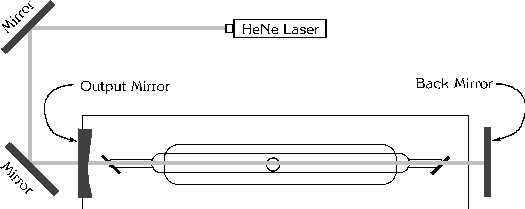
\includegraphics[width=0.7\linewidth]{images/CO24.png}}
        \caption{Alignment Configuration (note: diffraction grating not shown; it is between the back mirror and the right Brewster window)}
        \label{fig:AlignmentConfiguration}
    \end{figure}

    \item Turn on the red laser.

    \item Adjust the mirrors with the knobs until the red laser beam goes through the middle of the bore without reflecting off the walls of the tube. It will probably not look as if it goes through the middle of the Brewster windows, and it may not go exactly through the middle of the output mirror. Going down the center of the bore is the most important. Since the beam goes through those Brewster windows, the light that you will see on the paper blocking the back mirror will appear fairly diffuse.

    \item Now remove the paper blocking the back mirror and adjust the mirror so that the reflection is centered on the output port of the red HeNe laser (use the iris in front of the HeNe laser). Another good trick is to poke a small hole in a piece of white paper (this effectively makes an iris). With the lights off, hold this paper between the back mirror and the laser tube (where the diffraction grating is). If you line up the incoming beam with the small hole you have made, you will see the reflected beam on that piece of paper. Now twist the knobs on the back mirror to align the reflected beam with the hole where the incoming beam enters. This should get you more or less aligned with the output port of the HeNe laser. Also note that the light that makes it all the way back to the output port of the HeNe laser will have passes through the Brewster windows twice! Thus, it will appear very diffuse.
    
    \textbf{Checkpoint. Call the staff over to check the alignment of your back mirror.}

    \item Now re-install the output coupler mirror using the vinyl gloves. Now adjust the output coupler mirror so that the inner surface reflection of that mirror (the bigger, dimmer one of the two) is centered on the output port of the HeNe laser. Alignment is pretty much complete. \textbf{Note}: alignment does not need to be \emph{that} good to get the CO$_2$ laser to lase! Doing a fantastic job aligning the red laser is less important that doing a fantastic job optimizing the CO$_2$ laser. As long as the mirrors are aligned enough to allow some lasing to happen, you can optimize the laser by measuring the output with a power meter and tweaking the mirrors from there. Therefore, don't waste too much time doing this part perfectly. Don't be afraid to move ahead and learn how the gas system and water flow systems work. Get those going and see if your alignment needs more work. You can always come back and realign the HeNe laser.

    \item Block off the output port of the Red laser with a firebrick to protect it from the CO$_2$ beam. Place the power detector in front of the CO$_2$ output port and place a firebrick behind the detector. Place the power meter in Automatic mode and it will change scales automatically on the power meter scale. The remaining steps are turning on the water and turning on the gas. Read on below to learn to do those.

\end{enumerate}

\subsection{Pumping-Out and Filling the Laser Tube}

\begin{figure}[h]
    \centering
    \href{http://experimentationlab.berkeley.edu/sites/default/files/upimages/lasergaspic_small.jpg}{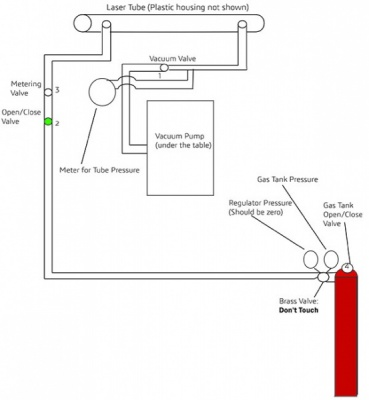
\includegraphics[width=0.5\linewidth]{images/lasergaspic_small.jpg}}
    \caption{Gas lines and Valves}
    \label{fig:GasLinesAndValves}
\end{figure}
 
Refer to the diagram above for the valve knob numbers.

\begin{enumerate}
    \item Make sure that the gas tank is open. If it is not, give knob number 4 a couple turns to the left, until the pressure meter attached to the tank indicates gas flow. Valve number 4 is silver. It is next to another valve that is brass and says do not touch. If you mess with that valve, you will blow the glass tube to smithereens. Therefore, do not touch that knob.
    
    \item Valves 2 and 3 control the amount of gas flow into the laser tube. 2 is the coarse adjustment. 3 is the finer adjustment. With your eye on the pressure meter, twist valve number 2. You will see the pressure meter spike up. Close it before it gets too high. You'll come back to this knob in the next step.
    
    \item Valve 1 is the vacuum valve. If the vacuum is too strong, it will pump out all of the gas coming in. Twist the knob to see how it affects the pressure. You must find a balance between the vacuum pump and the CO$_2$ pump such that the pressure in the tube stays at a constant value between 10mmHg and 15mmHg. Obviously, the wrong way to achieve the balance is to have a super high vacuum and high CO$_2$ flow because then you'll empty out the C0$_2$ tank (you pump in CO$_2$, then the vacuum pumps it right back out).  Thus, try and find a balance that minimizes the gas flow by \textbf{tweaking knobs 1, 2, and 3.}


\textbf{Checkpoint.  Have a staff member come and check your setup to make sure that the gas is flowing properly. Explain what each valve, number 1 to 4, does. Which valve should you never touch?}


    \item Before you begin, ask a GSI or staff for help. The pumping system is a molecular sieve; no cold trap of liquid Nitrogen ($LN_2$) is used. The molecular sieve keeps oil from migrating up into the laser system as you pump. Always keep a vacuum on the laser tube when not in use. There may be moisture in the laser tube that would cause the pressure to be affected making it difficult to pump down properly. \textbf{Note this is a gas flowing system.} See Figure \ref{fig:GasLinesAndValves} above. Gas flows into the top of the Green valve \#3 and Black metering valve \#1, (Note the metering valve is always open a small amount, you can not close it, it meters the gas flow) located at the end of the Laser Table nearest the door, then gas flows through the laser and then through valve \#6 to the vacuum system. The vacuum pump goes to the \#6 valve (see Figure \ref{fig:GasLinesAndValves}), vary the metering valve \#1 (this valve never closes it is always in some open condition) and Vacuum valve \#6 opening to regulate the pressure flow. This metering valve does not close and is used to regulate the pressure gas flow to the laser. When the valves are all the way in (turned clockwise) they are closed. \emph{\textbf{The metering valve is always open a little even when it is closed down.}} As you back out the screws (by turning them counter-clockwise), gas flows.

    \item Note you should look at the hook up for the vacuum system for the CO$_2$ laser. There has been changes and we use a flowing gas system. We first want to flush the system. Make sure that \emph{all valves are closed including the GAS TANK VALVE}. Make sure the pump is turned on. Then open valve \#6 and then valve \#2. (This cleans anything out of the gas tank regulator.)
\end{enumerate}

If you adjust the pressure to 10 mmHg and then close both \#6 and \#3, the tube should theoretically maintain that pressure. However, observe what happens over time if you do this? Discuss whether you need CO$_2$ gas to be flowing (and why) in order to do the experiment. You can adjust the pressure flow to about 10 mm by adjusting valve's \#3, \#6, and \#1 until the pressure on the gauge settles between 10 and 15 torr (mm Hg). Make sure that the flow is as small as reasonable otherwise you will empty the gas tank.

Question: based on your observation on how long it takes to pump out the gas tube when valve \#6 is maximally open and valve \#3 is closed, how long would it take to empty the gas bottle if you would settle for maximum flow?

\subsection{Power-On and -Off, and Maximizing Laser Power}

\begin{enumerate}
    \item Check that \textbf{all} electrical connections are secure to the equipment rack and to the laser. (See appendix at back of this write-up).

    \item Turn on the water as follows: There are two water valves by the door: the \textbf{blue} valve is in-flow, the \textbf{red }valve is out-flow. The idea is to protect the laser tube from the pressure of the water line. So when you turn the water off and on, make sure the out-flow valve is open whenever the in-flow valve is open. To turn the water on, start with both the red and blue valves closed.
    
    \textbf{Procedure for Water Turn on/off:} Turn on the water-supply faucet in 286 LeConte (across the hall, by the sink to your right as you walk in the door)-Pull down the \textbf{yellow lever} valve marked CO$_2$ Water to turn on the Water, \textbf{DO NOT Touch or turn} the flow valve above it; Then, go back in the room with the laser, The water interlock box is on the wall over the safety glasses. \textbf{Make sure the power to the interlock is turned on.} The power box is located directly to the left of the interlock box. To turn on the interlock: Push and hold the button, then open the Red and then open the BLUE valve. Now the Red light on the box will come on, indicating water is flowing. This completes the water turn on procedure. \textbf{To turn off the water} close the Blue valve 1st, then Red Valve, then go to 286 and push the CO$_2$ Water lever valve back (90 degrees) to close it.
    
    Put on your safety goggles located next to the water interlock Box. If the water stops flowing then this interlock will stop the water flow for safety. Always remember to turn off the BLUE 1st and then the RED when leaving the Laser for the day as stated above.
    
    \item \textbf{Procedure to change the gas pressure:} To Change the gas pressure do the following: \textbf{DO NOT Change the gas pressure while the high voltage is on}.  If the high voltage is on while you are changing the gas pressure, you will make a connection to the ground from touching the metal knobs/table, creating a potential difference and allowing the electricity run through you -- a potentially \textbf{LETHAL HAZARD} (at around 15,000 volts!). So, \textbf{Turn off}, then on, again the both regulator power switches quickly to disengage the interlock, i.e. the red light goes out. \emph{Always} turn off the high voltage before you change the pressure. Then you can adjust the gas pressure with the metering valve \#1 and the Vacuum valve \#6.
    
    \item Now for the high voltage (HV). Make sure that all of the plastic panels are securely fastened on the laser housing. The electrical connections are already made; High Voltage is connected to \#2 terminal at the center of the laser tube. The voltage is regulated by two Current Regulators. How does the laser work then?? The current regulators maintains a constant current through the CO$_2$ laser tube. The regulator controls the current by adjusting a current through a tetrode vacuum tube device and transistors inside the regulator. The current regulator is in series with the high voltage supply and the CO$_2$ laser tube. Changing the high voltage gets you nowhere, since it is the current that is regulated. Also, the high voltage power supply meter reads the total supply voltage only, not the voltage across the tube. The voltage across the laser tube equals the high voltage meter reading minus the voltage across the current regulator. (The voltage drop across the regulator is between 2kV and 6kV, see the meter scale switch on the current regulator).
    
    To start, turn on the two Regulators. Then make sure that the powerstat (variable transformer) knob on the High Voltage Power supply is all the way down to zero (CCW), then turn on the HV Power supply.
    
    After approximately 30 seconds, press the HV interlock button on the Regulators to allow current to flow. If you have satisfied all of the interlocks, the red light will come on. Set the current so that it reads around 7 mA on each regulator. This current is the internal regulator idle current until the laser tube breaks down (passes current).
    
    \textbf{*Remember do not exceed 10 mA MAXIMUM total current for each current regular.}
    
    \emph{Slowly} turn up the powerstat knob increasing the high voltage. You will see the voltage increase on the high voltage panel but not on the regulator panel. This is because the regulator does not allow current to flow until the voltage passes a threshold value. Continue to increase the voltage until you see the voltage reading on the regulator panel voltmeter jump up. Now the regulators allows current to flow through the laser tube (tube breaks down). You should at the same time see a pink-purple glow discharge in the laser tube itself. (This should happen at almost the maximum output voltage)

    \textbf{To turn off high voltage}

    \begin{enumerate}
        \item Flip the both regulator power switches off and then on. This cuts off HV power to the two halves of the laser tube.
    
        \item Turn HV down to zero. DO NOT TURN OFF REGULATORS YET!
        
        \item Wait until HV meter on High voltage power supply reads zero. Then shut off the HV power supply and regulators.
        
        \textbf{CAUTION}: The high voltage bleeds off slowly, so all points are still electrically hot for several minutes. Don't touch them without supervision or prior instruction.
        
        \item When you are done for the day, Shut off water, \textbf{first} the BLUE handle, then the RED handle, one right after the other, and then the supply faucet across the hall in room 286. Also turn off all power meters and detector and all other electrical devices \emph{except the vacuum pump}, which you should leave running with all valves closed in the vacuum lines, etc.
    \end{enumerate}
    
    \item If you have properly aligned the laser it should be now lasing, and you should see power on the power meter. Much more likely, though, is that you are not lasing yet, but are very close and need to make some fine adjustments. To start, record the micrometer settings on both the back mirror and on the output mirror so you can return to them if necessary. (Check equipment specs on how to read the micrometers)
    
    With the back mirror fixed, slowly tweak (ADJUST) the output mirror and watch the power meter for an increase in power. Use some scientific method here-one approach is to leave the vertical micrometer fixed and vary the horizontal position, then change the vertical slightly and again vary the horizontal, ``walking'' through the various orientations. After each mirror movement, it takes several seconds before the discharge and lasing power settle down. A continuous movement of the mirror, no matter how slowly you turn the knob, will completely mask the lasing action. Turn the knob a tad, wait a couple of seconds, turn it again, etc. This is true for adjusting both mirrors - be patient and wait for the discharge to settle down.
    
    If this doesn't work, return the micrometers to their original settings and then change the back mirror \emph{slightly}. Then again walk through the output mirror orientations. You will need to repeat this process until you see a power reading on the power meter.
    
    If this doesn't work, carefully shut off the high voltage SEE ABOVE ``\textbf{To turn off high voltage}'' and again turn on the 632 nm at 6 mW laser and make sure that the beam travels down the center of the tube, and that the return beam enters the He-Ne laser at the same point that the exiting beam does. It really is crucial here that the beam travels down the center of the laser tube.
    
    \item Assuming some output is obtained, maximize the power by adjusting the micrometers. Move them slowly, in small steps - step and wait, step and wait. It takes time for the power and power meter to adjust to changes. There is always some backlash. Try ``walking'' the beam across the bore by detuning the back mirror, and compensating for it in the front. Do this until a maximum is reached. You should be able to get at least 700 mW, and the more power you have the better-off you will be, especially when you try to use the grating. The laser is capable of putting out 10 watts. It may be desirable to write down these final micrometer settings for further use (like if the laser gets detuned somehow). If the laser doesn't lase the next time it is turned on, and everything else says it should, try adjusting the back mirror or grating first. Sometimes you will leave at 5 PM with the laser in operating condition, and will return the next day and find it not operating. Remember that temperatures of the laser parts have changed, and the adjustments may have changed, but these changes are slight, so have patience and make small adjustments while attempting to regain the proper operating conditions. You shouldn't have to start over. (Any problems, call the staff for sympathy and perhaps advice).
\end{enumerate}

\pagebreak

\section{Experiments}

Your report should have discussions and explanations of the data obtained in the following experiments.

\subsection{Current-voltage Curve and Gas Pressure}

Find the $V$-$I$ curve of the laser tube discharge as a function of gas pressure, for three different pressures. Limit the maximum pressure to 20 torr. Remember that when changing pressure you should have the \emph{\textbf{high voltage off.}}

\begin{figure}[h]
\centering
    \href{http://experimentationlab.berkeley.edu/sites/default/files/upimages/2_lasercircuitpic_small.jpg}{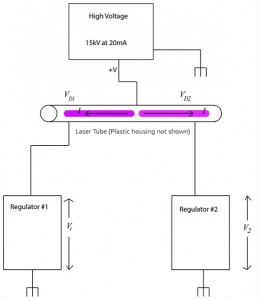
\includegraphics[width=0.5\linewidth]{images/2_lasercircuitpic_small.jpg}}
    \caption{}
\end{figure}

The diagram above shows the circuit layout of the system. From this, you should be able to understand how the readings on the high voltage source and the regulators determine the discharge tube voltage and current. Adjust the regulator currents to drop different voltages across the tube. Keep in mind that the power rating of the high voltage source is 20mA at 15kV. Requesting too much power from the high voltage source will result in a blown fuse. It's not the end of the world, but try to avoid that. The meters are accurate to 5\%. The top meter lacks notches, so use your eyeball to gauge the different current levels.

\subsection{Power Threshold}

Vary the input power to the discharge and observe when the laser starts lasing. How does the threshold depend on the gas pressure? How sensitive is it to the optical alignment? (Qualitative measurements in both cases).

\subsection{Output Power Stability}

How stable is the output power? Near the lasing threshold are the fluctuations larger or smaller? (Qualitative measurements).

\subsection{Laser Spectrum}

Use the spectrum analyzer to observe which wavelengths are present. This is the most important part of the lab. You will need the following information. Important note: it may be difficult to see the spectrum without single-frequency operation. Therefore, it may be necessary to move on to using the grating to improve the spectral density and then after alignment of the spectrometer return to this part.

\subsubsection{Beam-Finding}

\begin{itemize}
    \item The beam-finders used in this experiment come in a variety of shapes and sensitivities. But they all work the same way: They are coated with a material which fluoresces when exposed to ultra-violet light. Then as the laser-light hits the fluorescing coating, wherever the beam touches it, it ceases to glow. It absorbs heat and can burn up easily. Do Not Hold it there too long. More it around so that the screen does not burn.

    \item To use a beam finder, wear your safety glasses, turn on the UV lamp and point it at the beam finder. The beam finder will glow brightly. Slowly insert the beam finder into the beam region until a darkening of the surface is observed. That's it, you've found the beam.

    \item The higher the number, the more sensitive the beam finder. Beam finders \#7, and \#8 can easily be damaged by an incident laser beam of too great an intensity. If the beam spot turns completely dark remove the finder quickly. It should never be set up so you cannot remove it safely in less than 1 second.

    \item Toward that end, always use a firebrick as a backup surface.
\end{itemize}

\emph{\textbf{Use caution when inserting anything in the beam, especially any reflective or flammable object.}}

\subsubsection{The Spectrum Analyzer (Spectrometer)}

\begin{enumerate}
    \item Before you remove the power detector from the output port place a firebrick behind the detector to stop it from leaving the table area. Using the mirrors, direct the beam to near the spectrum analyzer input port. CAREFUL! Do not direct the beam to unintended directions! Wearing the UV safety glasses, use the UV lamp and a beam finder to locate the position of the beam. Then adjust the mirror and spectrum analyzer positions such that the beam enters the input slit.

    \item Make sure that the spectrum analyzer is level and in the same plane as the laser beam, then turn it on. Use a ruler to determine whether the spectrum analyzer is level relative to the top surface of the optical table (the bubble level on top of the analyzer is not reliable). Note that this turns on a UV lamp inside the unit, so you must continue to wear your safety glasses. Also make sure that the entrance slit is all the way open (adjusted by a knob on the back of the device). Then either open the viewing-lid on the top of the unit just enough to see inside (keeping as much room light out as possible). If you do not find a signal turn off the room lights and open the unit all the way.

    \item There is a beam finder inside the unit. Using the knob on the back, bring this beam finder into view and hold it perpendicularly to the horizontal. You should see a dark spot on the beam finder. Orient the beam or spectrometer so that this spot lies in the upper left quadrant of the beam finder brackets (see Figure \ref{fig:InsideTheSpectrometer}). Then lower the beam finder. Depending on which frequencies are lasing, you should see at least one spot or line under the appropriate wavelength indicator.
    \begin{figure}[h]
        \centering
        \href{http://experimentationlab.berkeley.edu/sites/default/files/images/CO26.gif}{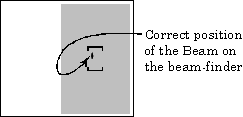
\includegraphics[width=0.5\linewidth]{images/CO26.png}}
        \caption{Inside the Spectrometer}
        \label{fig:InsideTheSpectrometer}
    \end{figure}
    
    How many lines are lasing simultaneously? Does the lasing spectrum change when the input power is increased from the threshold value, or when the gas pressure is changed, or when the table is pressed (press down on it with your thumb)?
    
    \textbf{Checkpoint. Call over a staff member and show them the signal line on the spectrum analyzer.}
    
    \item Replace the end mirror with the diffraction grating and measure the wavelengths and intensities of all possible lasing lines, as described below. First, shut off the laser power: for convenience we remind you of the procedure:
    
    \textbf{To turn off high voltage}
    
    \begin{enumerate}
        \item Flip the regulator power switch off and then on. This cuts off power to the laser.
    
        \item Turn HV down to zero. (CCW).
        
        \item Wait until HV meter reads nearly zero and then shut off the power supply and regulator.
    \end{enumerate}
    
    \textbf{CAUTION}: The high voltage bleeds off slowly, so all points are still electrically hot for several minutes. Don't touch them without supervision or prior instruction.
    
    \begin{figure}[h]
        \centering
        \href{http://experimentationlab.berkeley.edu/sites/default/files/images/CO27.gif}{
\includegraphics[width=0.5\linewidth]{images/CO27.png}}
        \caption{HeNe interference pattern}
        \label{fig:HeNeInterferencePattern}
    \end{figure}
    
    Swing the grating into place taking care not to touch its expensive optical surface. The grating functions in place of the back-mirror and will allow you to align the laser for one lasing wavelength at a time. Once again you will use the Red alignment laser as an alignment tool. Rotate the mirror as before and set the laser up as before and turn it on. Place a card with a small hole in it between the back Brewster window and the grating inside the large plastic safety box. When the Red beam passes through the hole and hits the grating, you can see the reflected diffraction pattern on the card (see Figure \ref{fig:HeNeInterferencePattern}). The row of dots should be horizontal, and as you move the grating, different dots should fall on top of the hole. Note that the dots are a little higher then the original laser beam. This is because the Grating is angled up a very small amount. You will need to adjust the output coupler mirror to compensate for this alignment. You should only have to adjust the grating by rotating its mount around the vertical axis (see Figure \ref{fig:TheLaserTopView}, \#5); the other orientations are fixed by what you do with the HeNe. If you cannot make the HeNe interference pattern horizontal, it is possible that the grating is not aligned along its other axes and you should see the staff for assistance. It does not help to turn the small allen-head screw that rotates the grating within its mount, don't do it. (THIS WILL CAUSE A LOSS OF TIME FOR YOU)
    
    Align the grating so that the reflected \emph{reference-dot} (see Figure \ref{fig:HeNeInterferencePattern}) returns to the output port of the HeNe laser. This grating angle is very close to the proper alignment for the P(20) line. You will have to adjust the grating slightly later since the diffraction pattern of the HeNe is only a measuring tool and this reference dot does not coincide exactly with the CO$_2$ P(20) line. Use a rubber band to hold the grating in position against the micrometer.
    
      \textbf{ Checkpoint. Call over a staff member and show them your P(20) line.}
    
    Again, protect the HeNe output port by blocking it with a fire brick. Turn on the CO$_2$ laser. Use the power meter and spectrometer to locate each line of the lasing spectrum as the grating angle is changed, and measure its intensity. You will need to tweak the alignment of the output coupler mirror in order to maximize your intensity. Keep the input-power constant during this process or you will be unable to compare intensities. You will have to develop a sensitive touch as you move the grating from one line to the next, tweaking it to maximize the output power before each measurement. Also, you will have to discern second order maxima from primary ones. This is by far the most time-consuming part of the lab AND THE MOST IMPORTANT PART. Have patience. There are two sets of lines, centered about 9.6 and 10.6 microns, perhaps 40 lines altogether.
   
    \begin{itemize}
        \item How is the threshold changed when the back mirror is replaced by the grating?
    
        \item Plot the maximum output power versus lasing wavelength.
        
    \textbf{Checkpoint. Call over a staff member to check out the spectrum.}
    
    \end{itemize}
    
    \item Lasing efficiency. Measure the output power for the P(18) and P(20) lines (10.57 and 10.59 microns) as a function of the input power. Plot the efficiency curves.
    
    \item Be sure to incorporate the answers to the following questions into the appropriate places of your report:
    
    \begin{itemize}
        \item What is a laser? What are the characteristics of its radiation?
    
        \item What is the principle of the CO$_2$ laser? Which are the relevant energy levels of CO$_2$ molecules? How are they excited to the upper lasing levels? Which transitions are the lasing transitions?
    
        \item Energy storage and energy transfer. How do nitrogen and helium in the gas mixture help increase the laser output?
    
        \item Last day of the experiment please fill out the \href{\ExperimentEvaluation}{\textbf{Experiment Evaluation}}
    
    \end{itemize}

\end{enumerate}

\pagebreak

\section{Apparatus Layout}

\begin{figure}[!h]
\centering
    \href{http://experimentationlab.berkeley.edu/sites/default/files/images/Co2_3.jpg}{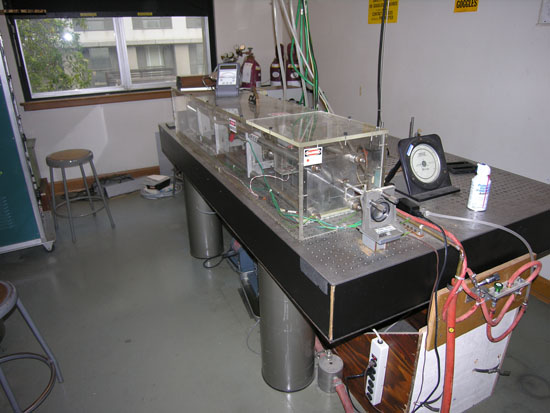
\includegraphics[width=0.8\linewidth]{images/Co2_3.jpg}} \\
    \caption{Room layout and air table for the Laser} system.
\end{figure}

\begin{figure}[!h]
\centering
    \href{http://experimentationlab.berkeley.edu/sites/default/files/images/Co2-29-new.png}{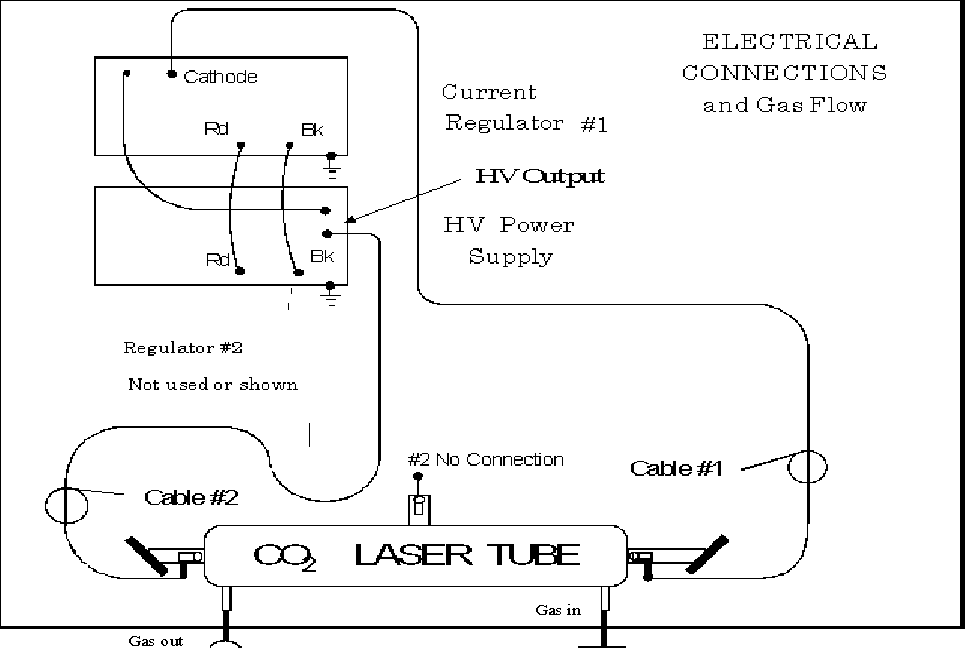
\includegraphics[width=0.6\linewidth]{images/Co2-29-new.png}} \\
    \caption{Connection diagram if only one current regulator is being used (Cable 2 is disconnected from the laser tube). The gray cable coming out of the front of the stack is an interlock cable that goes to the light on the door (to signify if the laser is on or not).}
\end{figure}

\begin{figure}[!h]
\centering
    \href{http://experimentationlab.berkeley.edu/sites/default/files/images/CO210.gif}{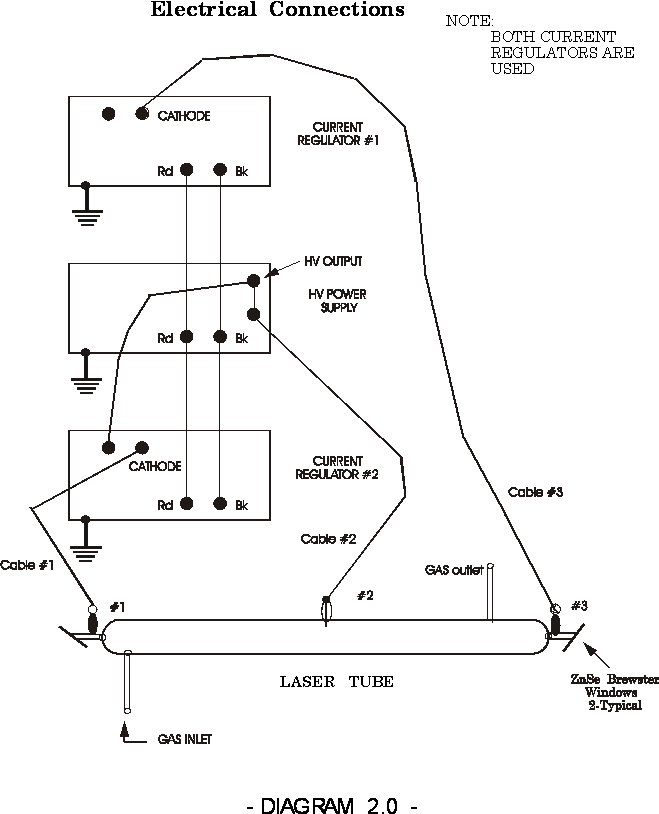
\includegraphics[width=0.4\linewidth]{images/CO210.png}} \\
    \caption{Connection diagram if two current regulators are being used. This will be the diagram to use most of the time, unless a regulator is getting repaired, etc. \textbf{This represents the currently used setup.}}
\end{figure}

\section{References}
\label{sec:References}

\begin{enumerate}
    \item Jenkins \& White. Ch. 17; ``The Diffraction Grating''. Fundamentals of Optics. 4th Ed. Pg 354-377. [\href{http://physics111.lib.berkeley.edu/Physics111/Reprints/CO2/OCR\%20ch.\%2017\%20the\%20diffraction\%20grating.pdf}{\textbf{Ch.17 Gratings}}]

    \item Gratings Data Sheet [\href{http://physics111.lib.berkeley.edu/Physics111/Reprints/CO2/grating.pdf}{\textbf{Grating Data Sheets}}]

    \item CO$_2$ Energy Levels [\href{http://physics111.lib.berkeley.edu/Physics111/Reprints/CO2/CO\_2\%20Energy\%20Levels.pdf}{\textbf{CO2 Energy Levels}}]

    \item F. Llewellyn, \emph{The Glow Discharge}, 1966. (In the Physics Library, the call number is \#QC711.L56)

    \item A. Howatson, \emph{An Introduction to Gas Discharges,} 2nd ed., 1976. (In the Physics Library, the call number is \#QC711.H78)

    \item C. Willett, \emph{Introduction to Gas Lasers: Population Inversion Mechanisms,} 1974. Gives detailed theoretical and experimental results, with a section devoted to CO$_2$ lasers.  (In the Physics Library, the call number is \#QC3.I625)

    \item {[\href{http://physics111.lib.berkeley.edu/Physics111/Reprints/CO2/CO2\_beam\_finder\_instructions.pdf}{\textbf{CO2 Beam Finder Specifications and Instructions}}]}

\end{enumerate}

Other reprints and reference materials can be found on the \href{http://physics111.lib.berkeley.edu/Physics111/Reprints/CO2/CO2\_index.html}{\textbf{Physics 111 Library Site}}

\end{document}
